% Options for packages loaded elsewhere
\PassOptionsToPackage{unicode}{hyperref}
\PassOptionsToPackage{hyphens}{url}
%
\documentclass[
  10pt,
  spanish,
]{article}
\usepackage{lmodern}
\usepackage{amssymb,amsmath}
\usepackage{ifxetex,ifluatex}
\ifnum 0\ifxetex 1\fi\ifluatex 1\fi=0 % if pdftex
  \usepackage[T1]{fontenc}
  \usepackage[utf8]{inputenc}
  \usepackage{textcomp} % provide euro and other symbols
\else % if luatex or xetex
  \usepackage{unicode-math}
  \defaultfontfeatures{Scale=MatchLowercase}
  \defaultfontfeatures[\rmfamily]{Ligatures=TeX,Scale=1}
  \setmainfont[]{Times New Roman}
\fi
% Use upquote if available, for straight quotes in verbatim environments
\IfFileExists{upquote.sty}{\usepackage{upquote}}{}
\IfFileExists{microtype.sty}{% use microtype if available
  \usepackage[]{microtype}
  \UseMicrotypeSet[protrusion]{basicmath} % disable protrusion for tt fonts
}{}
\makeatletter
\@ifundefined{KOMAClassName}{% if non-KOMA class
  \IfFileExists{parskip.sty}{%
    \usepackage{parskip}
  }{% else
    \setlength{\parindent}{0pt}
    \setlength{\parskip}{6pt plus 2pt minus 1pt}}
}{% if KOMA class
  \KOMAoptions{parskip=half}}
\makeatother
\usepackage{xcolor}
\IfFileExists{xurl.sty}{\usepackage{xurl}}{} % add URL line breaks if available
\IfFileExists{bookmark.sty}{\usepackage{bookmark}}{\usepackage{hyperref}}
\hypersetup{
  pdftitle={TMMS},
  pdfauthor={José Miguel Hernández Cabrera; Conrado Reyes Lafontaine; Carlos Alfredo Torres Cubilla},
  pdflang={es},
  hidelinks,
  pdfcreator={LaTeX via pandoc}}
\urlstyle{same} % disable monospaced font for URLs
\usepackage[left=2cm,right=2cm,top=2.25cm,bottom=2.25cm,headheight=12pt,letterpaper]{geometry}
\usepackage{longtable,booktabs}
% Correct order of tables after \paragraph or \subparagraph
\usepackage{etoolbox}
\makeatletter
\patchcmd\longtable{\par}{\if@noskipsec\mbox{}\fi\par}{}{}
\makeatother
% Allow footnotes in longtable head/foot
\IfFileExists{footnotehyper.sty}{\usepackage{footnotehyper}}{\usepackage{footnote}}
\makesavenoteenv{longtable}
\usepackage{graphicx,grffile}
\makeatletter
\def\maxwidth{\ifdim\Gin@nat@width>\linewidth\linewidth\else\Gin@nat@width\fi}
\def\maxheight{\ifdim\Gin@nat@height>\textheight\textheight\else\Gin@nat@height\fi}
\makeatother
% Scale images if necessary, so that they will not overflow the page
% margins by default, and it is still possible to overwrite the defaults
% using explicit options in \includegraphics[width, height, ...]{}
\setkeys{Gin}{width=\maxwidth,height=\maxheight,keepaspectratio}
% Set default figure placement to htbp
\makeatletter
\def\fps@figure{htbp}
\makeatother
\setlength{\emergencystretch}{3em} % prevent overfull lines
\providecommand{\tightlist}{%
  \setlength{\itemsep}{0pt}\setlength{\parskip}{0pt}}
\setcounter{secnumdepth}{-\maxdimen} % remove section numbering
\usepackage{caption}
\usepackage{float}
\usepackage{booktabs}
\usepackage{longtable}
\usepackage{array}
\usepackage{multirow}
\usepackage{wrapfig}
\usepackage{float}
\usepackage{colortbl}
\usepackage{pdflscape}
\usepackage{tabu}
\usepackage{threeparttable}
\usepackage{threeparttablex}
\usepackage[normalem]{ulem}
\usepackage{makecell}
\usepackage{xcolor}
\ifxetex
  % Load polyglossia as late as possible: uses bidi with RTL langages (e.g. Hebrew, Arabic)
  \usepackage{polyglossia}
  \setmainlanguage[]{spanish}
\else
  \usepackage[shorthands=off,main=spanish]{babel}
\fi

\title{TMMS}
\author{José Miguel Hernández Cabrera\footnote{Universidad de Salamanca,
  \href{mailto:idu008675@usal.es}{\nolinkurl{idu008675@usal.es}}} \and Conrado Reyes Lafontaine\footnote{Universidad de Salamanca,
  \href{mailto:correo@usal.es}{\nolinkurl{correo@usal.es}}} \and Carlos Alfredo Torres Cubilla\footnote{Universidad de Salamanca,
  \href{mailto:correo@usal.es}{\nolinkurl{correo@usal.es}}}}
\date{}

\begin{document}
\maketitle
\begin{abstract}
REDACTAR
\end{abstract}

\hypertarget{introducciuxf3n}{%
\section{Introducción}\label{introducciuxf3n}}

\textbf{CUIDADO} \emph{Toda la introducción son las instrucciones del
examen. Habrá que darle un cambio o rehacer la introducción}

Tradicionalmente, se evaluaba a los estudiantes a través de test de CI
para predecir su rendimiento académico y se consideraba que el CI era el
factor que mejor explicaba el rendimiento intelectual. Sin embargo,
actualmente, sabemos que nuestro equilibrio emocional y nuestra salud no
están relacionados con nuestro CI, sino que existen otras habilidades
emocionales y sociales que permiten nuestro ajuste social y relacional
(Gardner, 2001) y que tiene una incidencia clarísima sobre el éxito
académico, profesional y personal.

Según los autores Peter Salovey y John Mayers (1990), la inteligencia
emocional es la habilidad de las personas para atender y percibir los
sentimientos de forma apropiada y precisa, la capacidad para asimilarlos
y comprenderlos de forma adecuada y la destreza para regular y modificar
nuestro estado de ánimo.

Rafael Bisquerra (2003) ha aplicado la inteligencia emocional a la
educación, acuñando el término Educación Emocional para hacer referencia
a un proceso educativo, continuo y permanente, que pretende potenciar el
desarrollo emocional como complemento indispensable del desarrollo
cognitivo, constituyendo ambos los elementos esenciales del desarrollo
de la personalidad integra. Bisquerra considera que la educación
consiste en formar personas y no solo en impartir conocimientos. Además,
refiere que la educación debe ser para la vida y por ello debe responder
al desarrollo integral de los alumnos: social, moral y emocional. Del
mismo modo, considera que los profesores también deben ser
``emocionales''; es decir, que completen la enseñanza de competencias
cognitivas con competencias emocionales y sociales y que sepan gestionar
las emociones de la clase. Incluir la educación emocional y social en el
aula tiene múltiples beneficios para el alumno tales como orientar el
proceso de información, formar de manera integral para la vida y
favorecer las conductas sociales.

Bisquerra (2012) refiere que poseer inteligencia emocional significa
poner en práctica un conjunto de competencias emocionales que son los
conocimientos, capacidades, habilidades y actitudes necesarios para
comprender, expresar y regular de forma apropiada las emociones:

\begin{itemize}
\tightlist
\item
  Conciencia emocional: capacidad de tomar conciencia de las propias
  emociones y de los demás.
\item
  Regulación emocional: Capacidad para manejar las emociones de forma
  apropiada.
\item
  Autonomía emocional: capacidad para autogenerarse las emociones
  apropiadas en un momento determinado. Esto incluye una buena
  autoestima, actitud positiva hacia la vida y responsabilidad.
\end{itemize}

(Estas tres competencias formarían parte de la inteligencia
intrapersonal según la define Gardner)

\begin{itemize}
\tightlist
\item
  Habilidades socio-emocionales: capacidad para mantener unas buenas
  relaciones con los demás.
\item
  Habilidades para la vida y el bienestar emocional: comportamientos
  apropiados y responsables para afrontar los retos que se nos plantean
  y que nos permite organizar nuestra vida de forma sana y equilibrada,
  siendo capaces de generarse emociones positivas y relacionarse
  satisfactoriamente con los demás.
\end{itemize}

(Estas dos competencias formarían parte de la inteligencia interpersonal
según la define Gardner)

\hypertarget{muxe9todos}{%
\section{Métodos}\label{muxe9todos}}

\hypertarget{cuestionario}{%
\subsection{Cuestionario}\label{cuestionario}}

La Inteligencia Emocional puede evaluarse con el instrumento TMMS.

El TMMS-24 está basada en el Trait-Meta Mood Scale (TMMS) del grupo de
investigación Salovey y Mayer. La escala original es una escala que
evalúa el metaconocimiento de los estados emocionales mediante 48 ítems.
Fdez-Berrocal y col, propusieron una versión modificada del TMMS en
español, como resultado de previas investigaciones y propusieron una
versión simplificada, la TMMS de 24 ítems. Los ítems se miden en escala
Likert puntuados del 1 al 5, donde 1 es totalmente en desacuerdo y 5
representa estar totalmente de acuerdo con la proposición.

La TMMS contempla tres dimensiones de la Inteligencia Emocional:

\begin{itemize}
\tightlist
\item
  Atención: soy capaz de sentir y expresar los sentimientos de forma
  adecuada.
\item
  Claridad: comprendo bien mis estados emocionales.
\item
  Reparación: soy capaz de regular los estados emocionales
  correctamente.
\end{itemize}

El cuestionario es el siguiente:

\begin{longtable}[]{@{}l@{}}
\toprule
\begin{minipage}[b]{0.97\columnwidth}\raggedright
\textbf{TMMS-24}\strut
\end{minipage}\tabularnewline
\midrule
\endhead
\begin{minipage}[t]{0.97\columnwidth}\raggedright
INSTRUCCIONES: A continuación encontrará algunas afirmaciones sobre sus
emociones y sentimientos. Lea atentamente cada frase e indique, por
favor, el grado de acuerdo o desacuerdo con respecto a las mismas.
\textbf{Señale con una ``X'' la respuesta que más se aproxime a sus
preferencias.}\strut
\end{minipage}\tabularnewline
\begin{minipage}[t]{0.97\columnwidth}\raggedright
No hay respuestas correctas o incorrectas, ni buenas o malas. No emplee
mucho tiempo en cada respuesta.\strut
\end{minipage}\tabularnewline
\bottomrule
\end{longtable}

\begin{longtable}[]{@{}lllll@{}}
\toprule
\endhead
\begin{minipage}[t]{0.16\columnwidth}\raggedright
\textbf{1}: Nada de acuerdo\strut
\end{minipage} & \begin{minipage}[t]{0.16\columnwidth}\raggedright
\textbf{2}: Algo de acuerdo\strut
\end{minipage} & \begin{minipage}[t]{0.19\columnwidth}\raggedright
\textbf{3}: Bastante de acuerdo\strut
\end{minipage} & \begin{minipage}[t]{0.15\columnwidth}\raggedright
\textbf{4}: Muy de acuerdo\strut
\end{minipage} & \begin{minipage}[t]{0.21\columnwidth}\raggedright
\textbf{5}: Totalmente de acuerdo.\strut
\end{minipage}\tabularnewline
\bottomrule
\end{longtable}

\begin{table}[H]
\centering
\begin{tabular}{|>{}r|l|r|r|r|r|>{}r|}
\hline
No. & Pregunta &  &  &  &  & \\
\hline
1 & Presto mucha atención a los sentimientos. & 1 & 2 & 3 & 4 & 5\\
\hline
2 & Normalmente me preocupo mucho por lo que siento. & 1 & 2 & 3 & 4 & 5\\
\hline
3 & Normalmente dedico tiempo a pensar en mis emociones. & 1 & 2 & 3 & 4 & 5\\
\hline
4 & Pienso que merece la pena prestar atención a mis emociones y estado de ánimo. & 1 & 2 & 3 & 4 & 5\\
\hline
5 & Dejo que mis sentimientos afecten a mis pensamientos. & 1 & 2 & 3 & 4 & 5\\
\hline
6 & Pienso en mi estado de ánimo constantemente. & 1 & 2 & 3 & 4 & 5\\
\hline
7 & A menudo pienso en mis sentimientos. & 1 & 2 & 3 & 4 & 5\\
\hline
8 & Presto mucha atención a cómo me siento. & 1 & 2 & 3 & 4 & 5\\
\hline
9 & Tengo claros mis sentimientos. & 1 & 2 & 3 & 4 & 5\\
\hline
10 & Frecuentemente puedo definir mis sentimientos. & 1 & 2 & 3 & 4 & 5\\
\hline
11 & Casi siempre sé cómo me siento. & 1 & 2 & 3 & 4 & 5\\
\hline
12 & Normalmente conozco mis sentimientos sobre las personas. & 1 & 2 & 3 & 4 & 5\\
\hline
13 & A menudo me doy cuenta de mis sentimientos en diferentes situaciones. & 1 & 2 & 3 & 4 & 5\\
\hline
14 & Siempre puedo decir cómo me siento. & 1 & 2 & 3 & 4 & 5\\
\hline
15 & A veces puedo decir cuáles son mis emociones. & 1 & 2 & 3 & 4 & 5\\
\hline
16 & Puedo llegar a comprender mis sentimientos. & 1 & 2 & 3 & 4 & 5\\
\hline
17 & Aunque a veces me siento triste, suelo tener una visión optimista. & 1 & 2 & 3 & 4 & 5\\
\hline
18 & Aunque me sienta mal, procuro pensar en cosas agradables. & 1 & 2 & 3 & 4 & 5\\
\hline
19 & Cuando estoy triste, pienso en todos los placeres de la vida. & 1 & 2 & 3 & 4 & 5\\
\hline
20 & Intento tener pensamientos positivos aunque me sienta mal. & 1 & 2 & 3 & 4 & 5\\
\hline
21 & Si doy demasiadas vueltas a las cosas, complicándolas, trato de calmarme. & 1 & 2 & 3 & 4 & 5\\
\hline
22 & Me preocupo por tener un buen estado de ánimo. & 1 & 2 & 3 & 4 & 5\\
\hline
23 & Tengo mucha energía cuando me siento feliz. & 1 & 2 & 3 & 4 & 5\\
\hline
24 & Cuando estoy enfadado intento cambiar mi estado de ánimo. & 1 & 2 & 3 & 4 & 5\\
\hline
\end{tabular}
\end{table}

\addtocounter{table}{-2}

Para corregir y obtener una puntuación en cada uno de los factores, se
suman los ítems del 1 al 8 para el factor Atención Emocional, los ítems
del 9 al 16 para el factor Claridad Emocional y del 17 al 24 para el
factor Reparación de las emociones. Luego se compara la puntuación en
las tablas que muestran los puntos de corte para hombres y mujeres, pues
existen diferencias en las puntuaciones para cada uno de ellos.

\hypertarget{teoruxeda-de-respuesta-al-uxedtem}{%
\subsection{Teoría de respuesta al
ítem}\label{teoruxeda-de-respuesta-al-uxedtem}}

La información es el inverso de variabilidad. Es decir, a mayor
información, menor variabilidad.

\hypertarget{modelo-de-samejima}{%
\subsection{Modelo de Samejima}\label{modelo-de-samejima}}

\hypertarget{resultados}{%
\section{Resultados}\label{resultados}}

\hypertarget{descripciuxf3n}{%
\subsection{Descripción}\label{descripciuxf3n}}

Derivado del levantamiento del cuestionario, se recopilaron
originalmente 3595 observaciones. Además de los 24 reactivos, se
disponen de tres variables categóricas para identificar a grupos de
respondientes: profesión, sexo y rango de edad. No obstante, dado que
algunas observaciones de los reactivos presentaron inconsistencias y
valores perdimos, se decidió no contar con ellos dado que una imputación
podría crear inconsistencias metodológicas. Por lo tanto, quedaron 3153
observaciones. Cabe señalar que solamente se retiraron las filas
incompletas de los reactivos, por lo que en las variables categóricas
existen valores faltantes.

Por parte de los profesionales, el grupo mayoritario fueron 1,389
alumnos universitarios de Portugal (44.1\%), seguidos de 872 curas
(27.7\%), 421 personas que ni estudian ni trabajan (13.4\%), 367
profesores del estado mexicano de Colima (11.6\%) y, finalmente, 104
farmacéuticos (3.3\%).

El sexo de los respondientes se comprende de 1,818 hombres (58\%) y
1,323 mujeres (42\%), con 12 valores faltantes.

Por último, los rangos de edad se distribuyen de la siguiente manera: el
grupo mayoritario son 1,875 menores de 30 (59.5\%); le siguen 510 entre
30 y 40 (16.2\%), 400 de 41 a 50 (12.7\%) y 366 mayores a 50 (11.6\%),
así como 2 valores faltantes.

En cuanto a los reactivos, el cuadro \ref{tab:tab_tmms} muestra las
frecuencias relativas de las puntuaciones de cada ítem, por dimensión:

\begin{longtable}[]{@{}lrrrrrr@{}}
\caption{Frecuencias relativas de los reactivos del TMMS-24 por
dimensiones\label{tab:tab_tmms}}\tabularnewline
\toprule
Dimensiones & Item & 1 & 2 & 3 & 4 & 5\tabularnewline
\midrule
\endfirsthead
\toprule
Dimensiones & Item & 1 & 2 & 3 & 4 & 5\tabularnewline
\midrule
\endhead
Atención & 1 & 2.1 & 16.9 & 26.1 & 30.7 & 24.2\tabularnewline
& 2 & 3.7 & 19.5 & 26.7 & 29.5 & 20.5\tabularnewline
& 3 & 4.6 & 21.5 & 29.1 & 28.1 & 16.6\tabularnewline
& 4 & 2.6 & 13.7 & 28.4 & 32.1 & 23.2\tabularnewline
& 5 & 17.0 & 30.5 & 26.4 & 18.1 & 8.0\tabularnewline
& 6 & 19.7 & 31.6 & 25.2 & 16.1 & 7.5\tabularnewline
& 7 & 10.5 & 30.0 & 28.0 & 21.5 & 10.0\tabularnewline
& 8 & 7.8 & 24.6 & 29.4 & 25.4 & 12.7\tabularnewline
Claridad & 9 & 4.5 & 17.3 & 28.7 & 29.8 & 19.7\tabularnewline
& 10 & 4.4 & 19.2 & 30.4 & 30.7 & 15.3\tabularnewline
& 11 & 5.6 & 18.4 & 30.3 & 29.3 & 16.3\tabularnewline
& 12 & 3.6 & 17.8 & 32.4 & 31.3 & 14.9\tabularnewline
& 13 & 2.6 & 17.0 & 35.1 & 32.2 & 13.1\tabularnewline
& 14 & 10.5 & 24.6 & 30.6 & 22.3 & 12.0\tabularnewline
& 15 & 6.5 & 23.8 & 35.7 & 23.5 & 10.5\tabularnewline
& 16 & 4.2 & 19.0 & 32.5 & 30.9 & 13.4\tabularnewline
Reparación & 17 & 7.6 & 16.7 & 25.3 & 30.4 & 19.9\tabularnewline
& 18 & 5.4 & 16.9 & 26.2 & 31.5 & 19.9\tabularnewline
& 19 & 12.7 & 24.1 & 27.8 & 22.6 & 12.7\tabularnewline
& 20 & 5.7 & 16.9 & 27.7 & 29.0 & 20.7\tabularnewline
& 21 & 6.1 & 18.9 & 28.1 & 30.3 & 16.7\tabularnewline
& 22 & 2.5 & 13.0 & 27.6 & 33.2 & 23.6\tabularnewline
& 23 & 1.2 & 5.4 & 16.5 & 31.7 & 45.3\tabularnewline
& 24 & 4.2 & 16.4 & 28.4 & 30.7 & 20.2\tabularnewline
\bottomrule
\end{longtable}

\hypertarget{anuxe1lisis-de-las-caracteruxedsticas-psicomuxe9tricas-del-cuestionario-tmms}{%
\section{Análisis de las características psicométricas del cuestionario
TMMS}\label{anuxe1lisis-de-las-caracteruxedsticas-psicomuxe9tricas-del-cuestionario-tmms}}

\hypertarget{anuxe1lisis-factorial-exploratorio}{%
\subsection{Análisis factorial
exploratorio}\label{anuxe1lisis-factorial-exploratorio}}

\begin{figure}
\centering
\includegraphics{TMMS_files/figure-latex/corr-1.pdf}
\caption{Correlaciones entre ítems}
\end{figure}

\begin{longtable}[]{@{}llr@{}}
\caption{Pruebas de esfericidad\label{tab:tab_esfe}}\tabularnewline
\toprule
\endhead
Determinante & & 8.973E-7\tabularnewline
Medida Kaiser-Meyer-Olkin de adecuación de muestreo & &
0.930\tabularnewline
Prueba de esfericidad de Bartlett & Aprox. Chi-cuadrado &
43765.192\tabularnewline
& gl & 276\tabularnewline
& Sig. & 0.000\tabularnewline
\bottomrule
\end{longtable}

\begin{longtable}[]{@{}lrrrr@{}}
\caption{Comunalidades y
unicidades\label{tab:tab_comuni}}\tabularnewline
\toprule
& Extracción ACP & Inicial AF & Extracción AF &
Unicidades\tabularnewline
\midrule
\endfirsthead
\toprule
& Extracción ACP & Inicial AF & Extracción AF &
Unicidades\tabularnewline
\midrule
\endhead
A1 & 0.550 & 0.576 & 0.493 & 0.424\tabularnewline
A2 & 0.653 & 0.644 & 0.608 & 0.356\tabularnewline
A3 & 0.653 & 0.618 & 0.608 & 0.382\tabularnewline
A4 & 0.547 & 0.523 & 0.490 & 0.477\tabularnewline
A5 & 0.435 & 0.359 & 0.344 & 0.641\tabularnewline
A6 & 0.552 & 0.553 & 0.479 & 0.447\tabularnewline
A7 & 0.678 & 0.647 & 0.637 & 0.353\tabularnewline
A8 & 0.687 & 0.634 & 0.654 & 0.366\tabularnewline
C9 & 0.617 & 0.592 & 0.565 & 0.408\tabularnewline
C10 & 0.684 & 0.652 & 0.647 & 0.348\tabularnewline
C11 & 0.718 & 0.642 & 0.691 & 0.358\tabularnewline
C12 & 0.574 & 0.509 & 0.508 & 0.491\tabularnewline
C13 & 0.625 & 0.563 & 0.576 & 0.437\tabularnewline
C14 & 0.558 & 0.498 & 0.483 & 0.502\tabularnewline
C15 & 0.450 & 0.433 & 0.381 & 0.567\tabularnewline
C16 & 0.650 & 0.563 & 0.604 & 0.437\tabularnewline
R17 & 0.629 & 0.602 & 0.584 & 0.398\tabularnewline
R18 & 0.720 & 0.690 & 0.700 & 0.310\tabularnewline
R19 & 0.510 & 0.431 & 0.417 & 0.569\tabularnewline
R20 & 0.755 & 0.669 & 0.748 & 0.331\tabularnewline
R21 & 0.495 & 0.404 & 0.411 & 0.596\tabularnewline
R22 & 0.575 & 0.516 & 0.507 & 0.484\tabularnewline
R23 & 0.388 & 0.357 & 0.325 & 0.643\tabularnewline
R24 & 0.528 & 0.429 & 0.453 & 0.571\tabularnewline
\bottomrule
\end{longtable}

\begin{longtable}[]{@{}llrrr@{}}
\caption{Varianza total explicada\label{tab:tab_varexp}}\tabularnewline
\toprule
& & Factor 1 & Factor 2 & Factor 3\tabularnewline
\midrule
\endfirsthead
\toprule
& & Factor 1 & Factor 2 & Factor 3\tabularnewline
\midrule
\endhead
Autovalores iniciales & Total & 8.297 & 3.855 & 2.080\tabularnewline
& \% de varianza & 34.570 & 16.060 & 8.668\tabularnewline
& \% acumulado & 34.570 & 50.630 & 59.298\tabularnewline
\(\sum a_i^2\) de la extracción & Total & 7.852 & 3.418 &
1.643\tabularnewline
& \% de varianza & 32.718 & 14.243 & 6.846\tabularnewline
& \% acumulado & 32.718 & 46.962 & 53.807\tabularnewline
\(\sum a_i^2\) de la rotación & Total & 4.426 & 4.350 &
4.137\tabularnewline
& \% de varianza & 18.443 & 18.125 & 17.239\tabularnewline
& \% acumulado & 18.443 & 36.568 & 53.807\tabularnewline
\bottomrule
\end{longtable}

\begin{table}[H]

\caption{\label{tab:unnamed-chunk-11}Matrices derivadas de métodos de extracción}
\centering
\begin{tabular}[t]{lrrrrrrrrr}
\toprule
\multicolumn{1}{c}{ } & \multicolumn{3}{c}{Componentes Principales} & \multicolumn{6}{c}{Factorización de eje principal} \\
\cmidrule(l{3pt}r{3pt}){2-4} \cmidrule(l{3pt}r{3pt}){5-10}
\multicolumn{1}{c}{\textbf{ }} & \multicolumn{3}{c}{\textbf{Componentes}} & \multicolumn{3}{c}{\textbf{Factores con Varimax}} & \multicolumn{3}{c}{\textbf{Factores con Oblimin}} \\
\cmidrule(l{3pt}r{3pt}){2-4} \cmidrule(l{3pt}r{3pt}){5-7} \cmidrule(l{3pt}r{3pt}){8-10}
  & 1 & 2 & 3 & 1 & 2 & 3 & 1 & 2 & 3\\
\midrule
A1 & 0.543 & 0.503 & 0.040 & 0.524 & 0.466 & 0.040 & 0.123 & 0.640 & 0.041\\
A2 & 0.522 & 0.611 & 0.085 & 0.510 & 0.583 & 0.083 & 0.040 & 0.760 & 0.025\\
A3 & 0.516 & 0.616 & 0.088 & 0.505 & 0.588 & 0.087 & 0.032 & 0.763 & 0.024\\
A4 & 0.559 & 0.472 & 0.108 & 0.539 & 0.436 & 0.099 & 0.071 & 0.632 & 0.123\\
A5 & 0.237 & 0.611 & 0.080 & 0.224 & 0.538 & 0.067 & -0.081 & 0.612 & -0.092\\
A6 & 0.401 & 0.617 & 0.100 & 0.386 & 0.567 & 0.092 & -0.031 & 0.703 & -0.010\\
A7 & 0.485 & 0.658 & 0.102 & 0.476 & 0.633 & 0.101 & -0.010 & 0.800 & 0.006\\
A8 & 0.541 & 0.623 & 0.080 & 0.532 & 0.603 & 0.082 & 0.048 & 0.786 & 0.023\\
\addlinespace
C9 & 0.684 & -0.138 & -0.362 & 0.667 & -0.128 & -0.323 & 0.740 & 0.025 & 0.005\\
C10 & 0.707 & -0.117 & -0.414 & 0.696 & -0.111 & -0.387 & 0.823 & 0.036 & -0.057\\
C11 & 0.703 & -0.174 & -0.440 & 0.696 & -0.169 & -0.422 & 0.876 & -0.029 & -0.065\\
C12 & 0.653 & -0.089 & -0.374 & 0.632 & -0.081 & -0.320 & 0.708 & 0.059 & -0.029\\
C13 & 0.718 & -0.048 & -0.328 & 0.700 & -0.044 & -0.290 & 0.701 & 0.127 & 0.015\\
C14 & 0.604 & -0.277 & -0.341 & 0.583 & -0.252 & -0.283 & 0.679 & -0.113 & 0.072\\
C15 & 0.592 & -0.142 & -0.283 & 0.563 & -0.125 & -0.219 & 0.569 & 0.019 & 0.069\\
C16 & 0.708 & -0.201 & -0.329 & 0.693 & -0.189 & -0.296 & 0.737 & -0.018 & 0.075\\
\addlinespace
R17 & 0.613 & -0.430 & 0.260 & 0.599 & -0.409 & 0.241 & 0.134 & -0.123 & 0.699\\
R18 & 0.623 & -0.448 & 0.362 & 0.618 & -0.440 & 0.354 & 0.023 & -0.117 & 0.840\\
R19 & 0.525 & -0.197 & 0.442 & 0.502 & -0.179 & 0.364 & -0.107 & 0.097 & 0.678\\
R20 & 0.619 & -0.459 & 0.402 & 0.617 & -0.456 & 0.399 & -0.023 & -0.121 & 0.894\\
R21 & 0.556 & -0.236 & 0.362 & 0.530 & -0.212 & 0.292 & -0.004 & 0.056 & 0.630\\
R22 & 0.645 & -0.185 & 0.353 & 0.623 & -0.170 & 0.300 & 0.026 & 0.130 & 0.657\\
R23 & 0.557 & -0.139 & 0.241 & 0.526 & -0.121 & 0.183 & 0.095 & 0.114 & 0.472\\
R24 & 0.574 & -0.311 & 0.320 & 0.551 & -0.282 & 0.264 & 0.054 & -0.012 & 0.643\\
\bottomrule
\end{tabular}
\end{table}

\hypertarget{anuxe1lisis-factorial-confirmatorio}{%
\subsection{Análisis factorial
confirmatorio}\label{anuxe1lisis-factorial-confirmatorio}}

\begin{figure}

{\centering 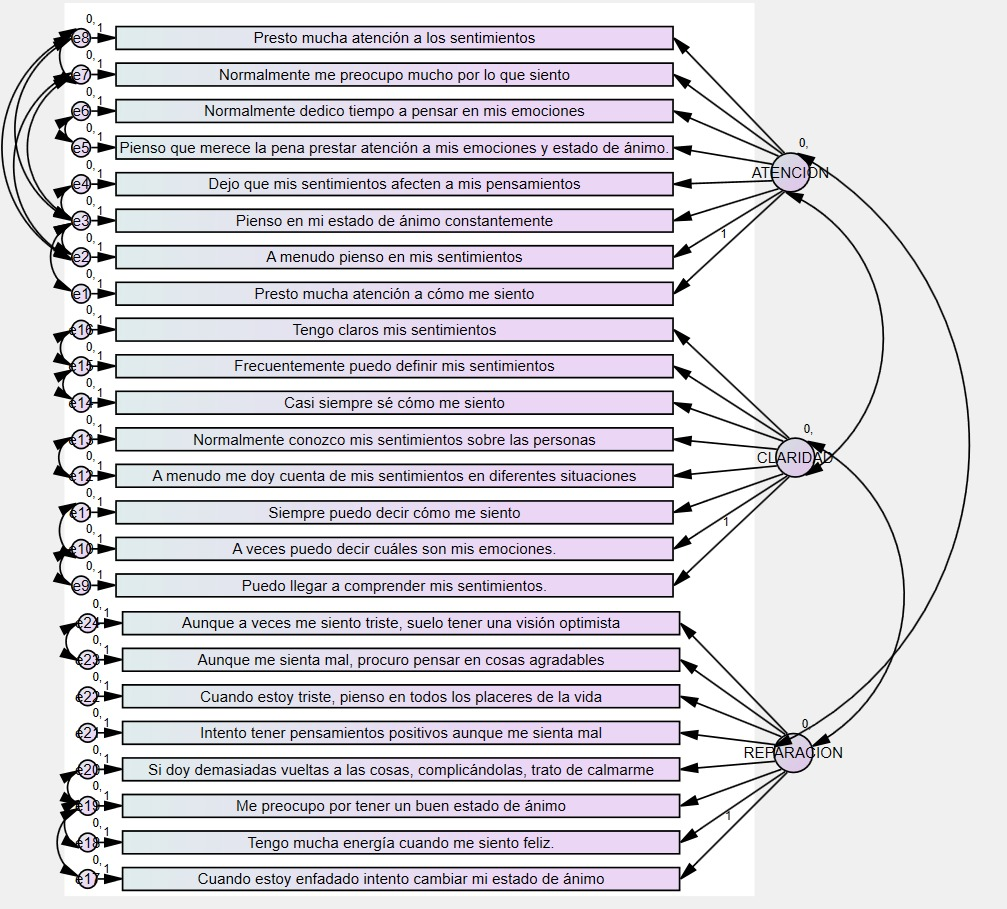
\includegraphics[width=0.8\linewidth]{./mapa_AMOS} 

}

\caption{Modelo confirmatorio del TMMS-24}\label{fig:unnamed-chunk-12}
\end{figure}

\hypertarget{capacidad-informativa-del-tmms}{%
\subsection{Capacidad informativa del
TMMS}\label{capacidad-informativa-del-tmms}}

\hypertarget{del-anuxe1lisis-factorial}{%
\subsubsection{Del análisis factorial}\label{del-anuxe1lisis-factorial}}

\begin{figure}
\centering
\includegraphics{TMMS_files/figure-latex/unnamed-chunk-14-1.pdf}
\caption{Curvas de información del análisis factorial}
\end{figure}

Observaciones del analisis factorial en las graficas, podemos ver con
las curvas de informacion de los items tienen importancias similares,
aunque encontramos items que presentan menos informacion como el A5, A6,
C14, C15, R19 y R23.

\hypertarget{de-la-teoruxeda-de-respuesta-del-uxedtem}{%
\subsubsection{De la Teoría de Respuesta del
Ítem}\label{de-la-teoruxeda-de-respuesta-del-uxedtem}}

\begin{figure}
\centering
\includegraphics{TMMS_files/figure-latex/unnamed-chunk-15-1.pdf}
\caption{Capacidad informativa del test}
\end{figure}

\break

\begin{figure}
\centering
\includegraphics{TMMS_files/figure-latex/unnamed-chunk-16-1.pdf}
\caption{Curvas características de los ítems por dimensión}
\end{figure}

Al dividir el TMMS en tres dimensiones vemos que en las tres se recoje
informacion de igual manera y con ayuda del paquete mirt podemos ver de
forma mas detalladas los items que menos recojen informacion en cada una
de estas.

Lo items con menos informacion por dimension:

\begin{itemize}
\tightlist
\item
  \emph{Atención}: A5 y A6
\item
  \emph{Claridad}: C12, C14 y C15
\item
  \emph{Recuperación}: R19, R21 y R23
\end{itemize}

\hypertarget{atenciuxf3n}{%
\subsubsection{Atención}\label{atenciuxf3n}}

factorización de matriz de correlaciones policóricas

Puntos de corte

Información

\hypertarget{capacidad-discriminante-de-cada-uxedtem}{%
\subsection{Capacidad discriminante de cada
ítem}\label{capacidad-discriminante-de-cada-uxedtem}}

\begin{longtable}[]{@{}lrlrlr@{}}
\caption{Parámetros de discriminación de los
ítems.\label{tab:tab_discr}}\tabularnewline
\toprule
& Atención & & Claridad & & Reparación\tabularnewline
\midrule
\endfirsthead
\toprule
& Atención & & Claridad & & Reparación\tabularnewline
\midrule
\endhead
A1 & 1.070 & C9 & 1.250 & R17 & 1.238\tabularnewline
A2 & 1.421 & C10 & 1.501 & R18 & 1.661\tabularnewline
A3 & 1.428 & C11 & 1.675 & R19 & 0.889\tabularnewline
A4 & 1.052 & C12 & 1.121 & R20 & 1.891\tabularnewline
A5 & 0.706 & C13 & 1.265 & R21 & 0.917\tabularnewline
A6 & 1.040 & C14 & 1.033 & R22 & 1.114\tabularnewline
A7 & 1.468 & C15 & 0.847 & R23 & 0.792\tabularnewline
A8 & 1.542 & C16 & 1.377 & R24 & 1.020\tabularnewline
\bottomrule
\end{longtable}

\hypertarget{atenciuxf3n-1}{%
\subsubsection{Atención}\label{atenciuxf3n-1}}

Discriminantes

Para cada ítem hay una única discriminación y varios parámetros de
dificultaddd correspondientes a las distintas categorías de las
variables.

\hypertarget{anuxe1lisis-de-las-categoruxedas-de-respuesta}{%
\subsection{Análisis de las categorías de
respuesta}\label{anuxe1lisis-de-las-categoruxedas-de-respuesta}}

\begin{figure}
\centering
\includegraphics{TMMS_files/figure-latex/unnamed-chunk-19-1.pdf}
\caption{Categorías de respuesta de los ítems por dimensión}
\end{figure}

En las gráficas de respuestas por items se aprecia que los items con
menos aportacion de informacion tienen de igual forma baja informacion
en la respuestas.

\hypertarget{anuxe1lisis-del-impacto-de-los-uxedtems}{%
\subsection{Análisis del impacto de los
ítems}\label{anuxe1lisis-del-impacto-de-los-uxedtems}}

\begin{table}[H]

\caption{\label{tab:unnamed-chunk-20}Tabla de impacto de los ítems}
\centering
\begin{tabular}[t]{lrrr}
\toprule
  & Frecuencia & Importancia & Impacto\\
\midrule
\textbf{A1} & \textbf{97.907} & \textbf{3.816} & \textbf{373.613}\\
A2 & 96.258 & 3.717 & 357.797\\
A3 & 95.401 & 3.580 & 341.569\\
\textbf{A4} & \textbf{97.431} & \textbf{3.821} & \textbf{372.288}\\
A5 & 83.000 & 3.115 & 258.520\\
\addlinespace
A6 & 80.304 & 3.068 & 246.378\\
A7 & 89.502 & 3.290 & 294.505\\
A8 & 92.198 & 3.471 & 319.991\\
\textbf{C9} & \textbf{95.496} & \textbf{3.587} & \textbf{342.571}\\
C10 & 95.592 & 3.547 & 339.058\\
\addlinespace
C11 & 94.355 & 3.537 & 333.719\\
C12 & 96.384 & 3.536 & 340.777\\
\textbf{C13} & \textbf{97.399} & \textbf{3.523} & \textbf{343.138}\\
C14 & 89.534 & 3.217 & 288.009\\
C15 & 93.530 & 3.312 & 309.763\\
\addlinespace
C16 & 95.845 & 3.495 & 334.945\\
R17 & 92.356 & 3.582 & 330.842\\
R18 & 94.608 & 3.592 & 339.863\\
R19 & 87.250 & 3.312 & 288.965\\
R20 & 94.291 & 3.578 & 337.357\\
\addlinespace
R21 & 93.879 & 3.509 & 329.375\\
\textbf{R22} & \textbf{97.463} & \textbf{3.781} & \textbf{368.479}\\
\textbf{R23} & \textbf{98.795} & \textbf{4.202} & \textbf{415.100}\\
R24 & 95.750 & 3.621 & 346.740\\
\bottomrule
\end{tabular}
\end{table}

Podemos discriminar algunos items segun la tabla tales como A5, A6, C14
y R19 ya que tienen los valores mas bajo de impacto.

\hypertarget{alfa-de-cronbach}{%
\subsection{Alfa de Cronbach}\label{alfa-de-cronbach}}

\begin{longtable}[]{@{}rrrr@{}}
\caption{Alfas de Cronbach.\label{tab:tab_cron}}\tabularnewline
\toprule
TMMS & Atención & Claridad & Reparación\tabularnewline
\midrule
\endfirsthead
\toprule
TMMS & Atención & Claridad & Reparación\tabularnewline
\midrule
\endhead
0.913 & 0.897 & 0.905 & 0.887\tabularnewline
\bottomrule
\end{longtable}

\hypertarget{discusiuxf3n-sobre-la-simplificaciuxf3n-del-cuestionario}{%
\section{Discusión sobre la simplificación del
cuestionario}\label{discusiuxf3n-sobre-la-simplificaciuxf3n-del-cuestionario}}

\begin{longtable}[]{@{}llll@{}}
\caption{Resumen.\label{tab:tab_discr}}\tabularnewline
\toprule
Dimension & AFE & TRI & Impacto\tabularnewline
\midrule
\endfirsthead
\toprule
Dimension & AFE & TRI & Impacto\tabularnewline
\midrule
\endhead
Atención & A5, A6 & A5, A6 & A5, A6\tabularnewline
Claridad & C14, C15 & C12, C14, C15 & C14\tabularnewline
Reparación & R19, R23 & R19, R21, R23 & R19\tabularnewline
\bottomrule
\end{longtable}

Mendiante la TRI se tiene una mayor discriminacion de Items en el
cuestionario de TMMS para las encuestas tomadas en este estudio, seguido
del AFE y la que meno discrimina es la tabla de Impacto.

\hypertarget{bibliografuxeda}{%
\section{Bibliografía}\label{bibliografuxeda}}

\end{document}
